%============================================================
\chapter{Procesamiento de la Señal de Batido}
\label{ch:procesamiento}
%============================================================

Los capítulos anteriores llegan hasta la salida del mezclador: una tensión
que, para cada blanco, oscila a una frecuencia de batido proporcional a su
distancia (ecuación~\eqref{eq:beat_freq}). Este capítulo describe todo lo que
pasa \textbf{desde que esa tensión se digitaliza hasta que aparece como una
fila del radargrama y una distancia en pantalla}. Es el núcleo del
procesamiento del sistema.

La cadena está repartida en dos lugares. En el microcontrolador
(\texttt{firmware/\allowbreak adquisicion/\allowbreak adquisicion.ino}) se muestrea, se filtra y se
diezma la señal, y se lee la triangular del generador. En la PC
(\texttt{analisis/\allowbreak vivo\_rapido.py} y \texttt{analisis/\allowbreak proceso\_rapido.py})
se reconstruye el sincronismo, se cortan las rampas, se corrige la no
linealidad del VCO, se calcula el espectro de cada rampa y se promedian
varias rampas para formar cada fila.

Cada etapa se presenta con su fundamento matemático, su implementación y lo
que se verificó de ella. La Tabla~\ref{tab:proc_parametros} reúne los valores
numéricos que se usan a lo largo del capítulo.

\begin{table}[H]
  \centering
  \caption{Parámetros de la cadena de procesamiento en el banco de
  laboratorio (generador con $T_c = 100\,\text{ms}$). Los valores medidos
  salen del encabezado de la captura de la placa a $90\,\text{cm}$ del
  28/09/2026.}
  \label{tab:proc_parametros}
  \begin{tabular}{llr}
    \toprule
    \textbf{Símbolo} & \textbf{Magnitud} & \textbf{Valor} \\
    \midrule
    $T_c$        & Período de la triangular (medido)      & $99{,}986\,\text{ms}$ \\
    $T_r = T_c/2$ & Duración de una rampa                & $49{,}993\,\text{ms}$ \\
    $F_\text{ADC}$ & Muestreo del PCM1808                 & $48\,000\,\text{sps}$ \\
    $M$          & Factor de diezmado                      & $8$ \\
    $F_s$        & Muestreo de salida                      & $6000\,\text{sps}$ \\
    $n$          & Muestras por rampa ($T_r F_s$)          & $300$ \\
    $N_\text{FFT}$ & Largo de la FFT (relleno $\times 8$)  & $2400$ \\
    $B$          & Ancho de banda barrido (curva del VCO)  & $1039{,}6\,\text{MHz}$ \\
    $\alpha_0 = B/T_r$ & Pendiente del barrido             & $2{,}079\times10^{10}\,\text{Hz/s}$ \\
    $2\alpha_0/c$ & Frecuencia de batido por metro         & $138{,}6\,\text{Hz/m}$ \\
    $\delta d = c/(2B)$ & Resolución en distancia          & $14{,}4\,\text{cm}$ \\
    $d_\text{max}$ & Alcance no ambiguo ($F_s/2$)          & $21{,}6\,\text{m}$ aparentes \\
    $N$          & Rampas por fila (por defecto)           & $8$ ($0{,}4\,\text{s}$) \\
    \bottomrule
  \end{tabular}
\end{table}

La pendiente $\alpha_0$ es la misma tasa de barrido $S = 2B/T_c$ del
Capítulo~\ref{ch:senal_if}: como cada rampa dura $T_r = T_c/2$,
$\alpha_0 = B/T_r = 2B/T_c$. En el código se la llama \texttt{alpha0}, y
así se la nombra en este capítulo.

%------------------------------------------------------------
\section{Visión general de la cadena}
\label{sec:proc_vision}

La Figura~\ref{fig:proc_cadena} muestra la cadena completa. Hay dos flujos
de datos que viajan juntos por el mismo puerto USB:

\begin{itemize}
  \item \textbf{El batido}: $6000$ muestras por segundo, ya filtradas y
    diezmadas en la placa. Es la señal que se mide.
  \item \textbf{La triangular}: una lectura del ADC del ESP32-C3 por cada
    bloque de DMA, unas $187{,}5$ por segundo. No se mide nada con ella:
    sirve para saber \emph{dónde empieza cada rampa}, o sea para reconstruir
    el sincronismo.
\end{itemize}

En la PC, un hilo dedicado vacía el puerto y separa los dos flujos. El hilo
del gráfico, cada $200\,\text{ms}$, toma todas las rampas completas que
llegaron, las procesa en lote y redibuja.

\begin{figure}[H]
  \centering
  \begin{tikzpicture}[
      font=\small,
      box/.style={draw, rounded corners, minimum height=0.8cm,
        minimum width=3.2cm, align=center, inner sep=3pt, fill=white},
      pc/.style={box, fill=blue!6},
      hw/.style={box, fill=orange!10},
      arr/.style={-{Latex[length=2mm]}, thick},
      node distance=5mm and 6mm
    ]
    % --- placa ---
    \node[hw] (pcm) {PCM1808\\$48\,000\,\text{sps}$};
    \node[hw, below=of pcm] (dec) {Antialias + diezmado $\times 8$\\
      (3 etapas de semibanda)};
    \node[hw, right=18mm of pcm] (gpio) {ADC del ESP32-C3\\(GPIO3, triangular)};
    \node[hw, below=of gpio] (lect) {Una lectura por\\bloque de DMA};
    \node[hw, below=12mm of $(dec.south)!0.5!(lect.south)$, minimum width=7.4cm]
      (usb) {USB: \texttt{batido} a $6000\,\text{sps}$ \;+\;
      \texttt{\#v,adc,índice} a $187{,}5/\text{s}$};
    \draw[arr] (pcm) -- (dec);
    \draw[arr] (gpio) -- (lect);
    \draw[arr] (dec) |- ($(usb.north)+(-1.8,0.45)$) -- ($(usb.north)+(-1.8,0)$);
    \draw[arr] (lect) |- ($(usb.north)+(1.8,0.45)$) -- ($(usb.north)+(1.8,0)$);
    % --- PC ---
    \node[pc, below left=8mm and -12mm of usb] (buf) {Buffer de batido};
    \node[pc, below right=8mm and -12mm of usb] (ajuste)
      {Ajuste de $T$ y $t_0$\\(últimos $5\,\text{s}$, cada $2\,\text{s}$)};
    \draw[arr] (usb.south) ++(-1.8,0) -- (buf.north);
    \draw[arr] (usb.south) ++(1.8,0) -- (ajuste.north);
    \node[pc, below=12mm of $(buf.south)!0.5!(ajuste.south)$] (corte)
      {Corte de la rampa $k$\\$n = 300$ muestras};
    \draw[arr] (buf) |- (corte.west);
    \draw[arr] (ajuste) |- node[pos=0.75, above, font=\scriptsize]
      {límites de rampa} (corte.east);
    \node[pc, below=of corte] (inv) {Bajadas: inversión temporal\\
      y resta de la media};
    \node[pc, below=of inv] (rem) {Remuestreo a $\theta$ uniforme\\
      + ventana de Hann (una matriz)};
    \node[pc, below=of rem] (fft) {FFT de $N_\text{FFT} = 2400$\\
      y magnitud $\lvert X_k\rvert$};
    \node[pc, below=of fft] (prom) {Promedio incoherente\\de $N$ rampas por fila};
    \node[pc, below=of prom] (fondo) {Resta del fondo, dB,\\
      detección y pico sub-bin};
    \node[pc, below=of fondo] (sal) {Radargrama, espectro\\y distancia};
    \draw[arr] (corte) -- (inv);
    \draw[arr] (inv) -- (rem);
    \draw[arr] (rem) -- (fft);
    \draw[arr] (fft) -- (prom);
    \draw[arr] (prom) -- (fondo);
    \draw[arr] (fondo) -- (sal);
    % --- marcos ---
    \node[draw, dashed, rounded corners, inner sep=6pt,
      fit=(pcm)(dec)(gpio)(lect), label={[font=\scriptsize\itshape]above:
      Placa (ESP32-C3 + PCM1808)}] {};
    \node[draw, dashed, rounded corners, inner sep=6pt,
      fit=(buf)(ajuste)(sal), label={[font=\scriptsize\itshape, anchor=south
      west]north west:PC (\texttt{vivo\_rapido.py})}] {};
    % --- secciones ---
    \node[font=\scriptsize, gray, right=3mm of dec]  {§\ref{sec:proc_diezmado}};
    \node[font=\scriptsize, gray, right=3mm of ajuste] {§\ref{sec:proc_sincronismo}};
    \node[font=\scriptsize, gray, right=3mm of inv]  {§\ref{sec:proc_rampa}};
    \node[font=\scriptsize, gray, right=3mm of rem]  {§\ref{sec:proc_theta}};
    \node[font=\scriptsize, gray, right=3mm of fft]  {§\ref{sec:proc_fft}};
    \node[font=\scriptsize, gray, right=3mm of prom] {§\ref{sec:proc_promedio}};
    \node[font=\scriptsize, gray, right=3mm of fondo]{§\ref{sec:proc_fondo}};
  \end{tikzpicture}
  \caption{Cadena de procesamiento completa. En naranja lo que corre en la
  placa; en azul lo que corre en la PC. A la derecha de cada bloque, la
  sección donde se describe.}
  \label{fig:proc_cadena}
\end{figure}

%------------------------------------------------------------
\section{Adquisición: sobremuestreo y diezmado}
\label{sec:proc_diezmado}

\subsection{El problema del aliasing}

Muestrear a $F_s$ sólo representa sin ambigüedad las frecuencias por debajo
de $F_s/2$. Cualquier componente por encima se \emph{pliega}: una frecuencia
$f > F_s/2$ aparece en $\lvert f - kF_s\rvert$ para el $k$ que la lleva a
$[0, F_s/2]$. En un radar FMCW eso es especialmente grave, porque la
frecuencia \emph{es} la distancia: un tono plegado se ve exactamente igual
que un blanco real a una distancia que no existe.

Para una rampa de $50\,\text{ms}$ alcanza con $F_s = 6000\,\text{sps}$:
con $138{,}6\,\text{Hz/m}$, el Nyquist de $3000\,\text{Hz}$ corresponde a
$21{,}6\,\text{m}$ aparentes, holgadamente más allá de cualquier blanco del
banco. Pero muestrear \emph{directamente} a $6000\,\text{sps}$ exigiría un
filtro antialias analógico que dejara pasar hasta $\sim 2{,}5\,\text{kHz}$ y
eliminara todo por encima de $3\,\text{kHz}$: una transición de pocos cientos
de hertz, que en analógico es cara, sensible a tolerancias y con mucha
distorsión de fase.

\subsection{La solución: muestrear rápido y filtrar en digital}

El PCM1808 muestrea a $F_\text{ADC} = 48\,000\,\text{sps}$, ocho veces más
de lo necesario (\emph{sobremuestreo}). A esa tasa el Nyquist está en
$24\,\text{kHz}$ y el antialias analógico es trivial; de hecho ya lo resuelve
internamente el propio PCM1808, con su filtro analógico y el sobremuestreo
$64\times$ de su modulador $\Delta\Sigma$
(Sección~\ref{sec:diagrama_bloques}). Después, el ESP32-C3 hace en digital
el filtrado abrupto que en analógico era difícil y recién entonces reduce la
tasa (\emph{diezmado}).

Diezmar por $M$ es quedarse con una de cada $M$ muestras de la señal ya
filtrada:
\begin{equation}
  y[m] = \sum_{i} h[i]\, x[Mm - i],
  \label{eq:proc_diezmado}
\end{equation}
y su espectro es la suma de $M$ copias desplazadas del espectro filtrado
\cite{Crochiere1983, Proakis2006}:
\begin{equation}
  Y\!\left(e^{j\omega}\right) = \frac{1}{M}\sum_{k=0}^{M-1}
  H\!\left(e^{j(\omega - 2\pi k)/M}\right)
  X\!\left(e^{j(\omega - 2\pi k)/M}\right).
  \label{eq:proc_alias}
\end{equation}
Las copias con $k \neq 0$ son el aliasing. Desaparecen sólo si
$H(e^{j\omega}) \approx 0$ para $\lvert\omega\rvert > \pi/M$: el filtro
$h$ \emph{es} el antialias, y su calidad decide cuánto se pliega.

\subsection{Por qué el promedio simple no alcanza}

La primera versión del firmware diezmaba promediando $M$ muestras, que es un
filtro $h[i] = 1/M$ de respuesta
$\lvert H(e^{j\omega})\rvert = \lvert\sin(M\omega/2)/(M\sin(\omega/2))\rvert$.
Sus lóbulos laterales caen muy despacio: un tono de $5\,\text{kHz}$ se
plegaba sobre $1\,\text{kHz}$ de la salida atenuado apenas $14\,\text{dB}$.
En la captura del banco había energía hasta el Nyquist mismo, que es
justamente la firma de algo plegándose.

\subsection{Cascada de filtros de semibanda}

El firmware actual divide por $8$ en tres etapas de $\times 2$
(Figura~\ref{fig:proc_semibanda}), cada una con un \textbf{filtro de
semibanda} de $L = 31$ coeficientes. Un filtro de semibanda es un FIR
simétrico que corta exactamente en la mitad de su Nyquist y cuya respuesta
cumple
\begin{equation}
  H\!\left(e^{j\omega}\right) + H\!\left(e^{j(\pi-\omega)}\right) = 1
  \label{eq:proc_semibanda}
\end{equation}
(en fase cero). En el dominio del tiempo eso equivale a que el coeficiente
central vale $1/2$ y \textbf{todos los coeficientes pares respecto del
centro son cero}, salvo el central: de los $31$, $14$ son ceros exactos
\cite{Crochiere1983}. Además, como cada etapa descarta la mitad de sus
salidas, sólo se calculan las que se conservan. El costo total es de
$\sim 1{,}3$ millones de multiplicaciones por segundo, alrededor del
$7$\,\% del microcontrolador.

\begin{figure}[H]
  \centering
  \begin{tikzpicture}[
      font=\small,
      box/.style={draw, rounded corners, minimum height=0.9cm,
        minimum width=1.6cm, align=center, fill=orange!10},
      dn/.style={draw, circle, inner sep=1pt, minimum size=0.8cm},
      arr/.style={-{Latex[length=2mm]}, thick},
      node distance=5mm
    ]
    \node (in) {$x[n]$};
    \node[box, right=of in] (h1) {$H_\text{sb}$};
    \node[dn, right=of h1] (d1) {$\downarrow 2$};
    \node[box, right=of d1] (h2) {$H_\text{sb}$};
    \node[dn, right=of h2] (d2) {$\downarrow 2$};
    \node[box, right=of d2] (h3) {$H_\text{sb}$};
    \node[dn, right=of h3] (d3) {$\downarrow 2$};
    \node[right=of d3] (out) {$y[m]$};
    \draw[arr] (in) -- (h1);  \draw[arr] (h1) -- (d1);
    \draw[arr] (d1) -- (h2);  \draw[arr] (h2) -- (d2);
    \draw[arr] (d2) -- (h3);  \draw[arr] (h3) -- (d3);
    \draw[arr] (d3) -- (out);
    \node[below=1mm of in,  font=\scriptsize] {$48\,\text{k}$};
    \node[below=1mm of $(d1)!0.5!(h2)$, font=\scriptsize] {$24\,\text{k}$};
    \node[below=1mm of $(d2)!0.5!(h3)$, font=\scriptsize] {$12\,\text{k}$};
    \node[below=1mm of out, font=\scriptsize] {$6\,\text{k}$};
  \end{tikzpicture}
  \caption{Diezmado $\times 8$ en tres etapas de semibanda. Cada etapa
  elimina todo lo que se plegaría en la división por dos siguiente.}
  \label{fig:proc_semibanda}
\end{figure}

La Tabla~\ref{tab:proc_rechazo} compara el rechazo de las dos soluciones
para tonos que caerían plegados sobre la banda útil.

\begin{table}[H]
  \centering
  \caption{Atenuación de los tonos que se pliegan sobre cada frecuencia de
  la salida, a $48\,\text{kHz}$ con $M = 8$.}
  \label{tab:proc_rechazo}
  \begin{tabular}{rcc}
    \toprule
    \textbf{Frecuencia de salida} & \textbf{Promedio de 8} &
      \textbf{Cascada de semibanda} \\
    \midrule
    $500\,\text{Hz}$  & $-20{,}7\,\text{dB}$ & $-90{,}5\,\text{dB}$ \\
    $1000\,\text{Hz}$ & $-14{,}2\,\text{dB}$ & $-87{,}4\,\text{dB}$ \\
    $2000\,\text{Hz}$ & $-7{,}6\,\text{dB}$  & $-71{,}1\,\text{dB}$ \\
    \bottomrule
  \end{tabular}
\end{table}

Por encima de $2400\,\text{Hz}$ el rechazo se degrada: es la banda de
transición de la última etapa, simétrica alrededor de $3000\,\text{Hz}$ por
la propiedad~\eqref{eq:proc_semibanda}. \textbf{La banda limpia va de $0$ a
$2400\,\text{Hz}$}, que a $138{,}6\,\text{Hz/m}$ son $17{,}3\,\text{m}$
aparentes. El rizado en esa banda es de $0{,}004\,\text{dB}$ y la ganancia en
continua es exactamente $1$: los coeficientes están en formato Q30 y suman
$2^{30}$ exacto. El código del filtro se verificó compilándolo con
\texttt{gcc} contra una referencia en Python, con coincidencia bit a bit.

\subsection{Ganancia de relación señal a ruido}

El sobremuestreo tiene además un beneficio de ruido. Si el ruido que llega al
ADC es blanco hasta $24\,\text{kHz}$, su potencia se reparte en $F_\text{ADC}/2$;
el filtro conserva sólo $F_s/2$ de ese ancho y descarta el resto en lugar de
plegarlo sobre la banda. La mejora es
\begin{equation}
  \Delta\text{SNR} = 10\log_{10}\frac{F_\text{ADC}}{F_s}
  = 10\log_{10} 8 \approx 9\,\text{dB}.
\end{equation}
Esta cuenta vale para el ruido de banda ancha. El ruido que ya está
\emph{dentro} de la banda útil no cambia.

\subsection{El precio: retardo de grupo}

Un FIR simétrico de $L$ coeficientes retrasa la señal $(L-1)/2$ muestras de
\emph{su propia} entrada. Referido a $48\,\text{kHz}$, la cascada retrasa
\begin{equation}
  \tau_\text{FIR} = 15\,(1 + 2 + 4) = 15\,(M-1) = 105 \text{ muestras}
  = 2{,}19\,\text{ms} \approx 13 \text{ muestras de salida}.
\end{equation}
Eso importa para el sincronismo: la triangular se lee en tiempo real, pero
la muestra de batido que sale en ese instante corresponde a $2{,}2\,\text{ms}$
antes. Sin compensarlo, los límites de rampa quedan corridos un $4{,}4$\,\%
de una rampa de $50\,\text{ms}$. El firmware suma ese retardo al índice que
emite con cada lectura de la triangular y lo informa con la línea
\texttt{\# retardo = 13 muestras}.

%------------------------------------------------------------
\section{Sincronismo a partir de la triangular}
\label{sec:proc_sincronismo}

\subsection{Qué hace falta y qué hay}

La FFT de la Sección~\ref{sec:proc_fft} se aplica a \emph{una rampa por
vez}. Para cortarlas hay que saber en qué muestra de batido empieza cada
una: eso es el sincronismo. El generador de laboratorio tiene una salida de
sincronismo, pero no entrega señal en este banco. En su lugar, la propia
triangular que sintoniza el VCO se lleva, a través de un divisor
$4{,}7\,\text{k}\Omega/4{,}7\,\text{k}\Omega$, al ADC del ESP32-C3 en GPIO3.

El firmware lee ese pin una vez por bloque de DMA, de $256$ muestras a
$48\,\text{kHz}$, o sea $187{,}5$ lecturas por segundo, y emite
\texttt{\#v,<adc>,<índice>}. El índice es la muestra de batido que
corresponde a ese instante, ya corregida por el retardo del filtro. Así las
dos señales quedan en la \textbf{misma escala de tiempo}.

Con $T_c = 100\,\text{ms}$ eso da apenas $\sim 19$ lecturas por período:
muy pocas para ubicar cada vértice de forma individual. Por eso el
sincronismo \textbf{no se detecta vértice por vértice}, sino que se
\textbf{ajusta un modelo} a muchos períodos a la vez.

\subsection{Modelo y ajuste}

Se modela la triangular leída como
\begin{equation}
  v(t) = A\,\Lambda\!\left(\frac{t - t_0}{T}\right) + \bar v + \text{ruido},
  \label{eq:proc_modelo_tri}
\end{equation}
donde $\Lambda(u)$ es la onda triangular de período $1$ con mínimo en
$u = 0$, $T$ es el período completo y $t_0$ el instante de un mínimo, o sea
el comienzo de una subida. $\Lambda$ es par, y su serie de Fourier tiene
sólo armónicos impares:
\begin{equation}
  \Lambda(u) = \frac{1}{2} - \frac{4}{\pi^2}\sum_{k\ \text{impar}}
  \frac{\cos(2\pi k u)}{k^2}.
  \label{eq:proc_serie_tri}
\end{equation}

El ajuste tiene dos pasos.

\paragraph{1. Búsqueda gruesa del período, sin suponer nada.}
Las lecturas se interpolan a una grilla uniforme, se les resta la media y
se calcula su FFT con ventana de Hann. El período es la inversa del máximo
espectral entre $1/200\,\text{ms}$ y $1/12\,\text{ms}$
(\texttt{buscar\_periodo()}). No hay riesgo de engancharse en un armónico:
por~\eqref{eq:proc_serie_tri} la triangular no tiene segundo armónico y el
tercero tiene $1/9$ de la amplitud del primero.

Este paso existe por un error que ya ocurrió. Una versión anterior buscaba
sólo $\pm 25$\,\% alrededor del período nominal; el período real quedaba
afuera y el ajuste devolvía un submúltiplo estable, preciso y falso.

\paragraph{2. Refinamiento del período y la fase.}
Se maximiza la magnitud del primer armónico
\begin{equation}
  S(T) = \sum_{i} \bigl(v_i - \bar v\bigr)\, e^{-j2\pi t_i/T}
  \label{eq:proc_armonico}
\end{equation}
sobre las lecturas $(t_i, v_i)$ de los últimos $5\,\text{s}$, unos $50$
períodos. El período que maximiza $\lvert S(T)\rvert$ es el que pone en fase
a todos los períodos de la ventana a la vez. Primero se recorre una grilla
de $\pm 1$\,\% alrededor del valor anterior ($\pm 10$\,\% alrededor de la
búsqueda gruesa, la primera vez), con cuatro puntos por lóbulo
principal; el lóbulo mide $\sim 1/N_\text{per}$ en valor relativo. Después
se refina con sección áurea dentro de $\pm 1$ paso de la grilla.

Con el período fijado, la fase sale del argumento de $S$. Reemplazando el
modelo~\eqref{eq:proc_modelo_tri} en~\eqref{eq:proc_armonico} y
conservando el primer armónico de~\eqref{eq:proc_serie_tri}:
\begin{equation}
  S(T) \approx \frac{N_\text{lect}}{2}\, A\, c_1\,
  e^{-j2\pi t_0/T},
  \qquad c_1 = -\frac{4}{\pi^2} < 0,
\end{equation}
y como $c_1$ es negativo,
\begin{equation}
  \arg S = \pi - \frac{2\pi t_0}{T}
  \quad\Longrightarrow\quad
  t_0 = \frac{T}{2\pi}\bigl(\pi - \arg S\bigr) \bmod T.
  \label{eq:proc_fase}
\end{equation}
El signo importa. Invertirlo devuelve $T - t_0$ en lugar de $t_0$, o sea
toma la bajada por subida, y no se nota en ningún otro número porque el
período sale bien igual.

\paragraph{Por qué un ajuste global.}
Ajustar un solo período a $50$ períodos usa toda la ventana como brazo de
palanca: el error de $T$ se reparte entre todas las lecturas en vez de
depender de un vértice. Sobre triangulares sintéticas a $100\,\text{ms}$, el
período sale con un error de $\sim 17\,\text{ppm}$ y el vértice con
$\sim 12\,\mu\text{s}$, contra $167\,\mu\text{s}$ de una muestra de batido.
El ajuste vectorizado tarda $4\,\text{ms}$ contra $105\,\text{ms}$ de la
versión original, y da el mismo período dentro de $5\,\text{ppm}$.

\paragraph{Por qué se rehace cada 2 s.}
El inicio de la rampa $k$ se calcula multiplicando el período por $k$, así
que un error residual $\delta T$ produce un error de límite que crece
linealmente desde el último ajuste:
\begin{equation}
  \delta t_k = \delta t_0 + k\,\frac{\delta T}{2}.
\end{equation}
Medido con $200\,\text{ppm}$ de deriva de reloj, el error de límite es de
$9\,\mu\text{s}$ ($0{,}05$\,\% de la rampa) con reajuste cada $2\,\text{s}$,
y de $1095\,\mu\text{s}$ ($5{,}4$\,\%) a los $60\,\text{s}$ sin reajuste.

\subsection{Límites de rampa}

Con $T$ y $t_0$, la rampa $k$ empieza en la muestra
\begin{equation}
  m_k = \operatorname{round}\!\Bigl[\Bigl(t_0 + k\,\frac{T}{2}\Bigr) F_s\Bigr],
  \qquad
  n = \operatorname{round}\!\Bigl(\frac{T}{2}\, F_s\Bigr) = 300,
  \label{eq:proc_limites}
\end{equation}
con $k$ par para las subidas y $k$ impar para las bajadas
(Figura~\ref{fig:proc_rampas}). El largo $n$ tiene histéresis: se cambia
sólo si $TF_s/2$ se aleja más de $0{,}6$ muestras del valor vigente, para
que todos los perfiles tengan el mismo largo.

\begin{figure}[H]
  \centering
  \begin{tikzpicture}[font=\small, x=1.45cm, y=1cm]
    % triangular
    \draw[->] (0,0) -- (8.4,0) node[right] {$t$};
    \draw[->] (0,0) -- (0,2.4) node[above] {$v(t)$};
    \draw[thick, orange!80!black]
      (0,0.2) -- (2,2) -- (4,0.2) -- (6,2) -- (8,0.2);
    % lecturas de la triangular (una cada ~0,21 unidades)
    \foreach \x in {0.1,0.31,...,7.9} {
      \pgfmathsetmacro{\ph}{mod(\x,4)}
      \pgfmathsetmacro{\y}{0.2+0.9*min(\ph,4-\ph)}
      \pgfmathsetmacro{\e}{0.09*sin(\x*977)}
      \fill[red!70!black] (\x,\y+\e) circle (1.3pt);
    }
    % limites de rampa
    \foreach \x/\k/\t in {0/0/subida, 2/1/bajada, 4/2/subida, 6/3/bajada} {
      \draw[dashed, gray] (\x,0) -- (\x,2.2);
      \node[font=\scriptsize] at (\x+1,2.35) {$k=\k$};
      \node[font=\scriptsize, gray] at (\x+1,-0.3) {\t};
    }
    \draw[dashed, gray] (8,0) -- (8,2.2);
    \node[below, font=\scriptsize] at (0,-0.45) {$t_0$};
    \draw[<->] (0,-0.75) -- node[below, font=\scriptsize] {$T/2$} (2,-0.75);
    \draw[<->] (4,-0.75) -- node[below, font=\scriptsize] {$T$} (8,-0.75);
    % bloques de batido
    \foreach \x/\c in {0/blue!10, 2/green!12, 4/blue!10, 6/green!12} {
      \draw[fill=\c] (\x+0.05,-2.1) rectangle (\x+1.95,-1.4);
    }
    \foreach \x in {0,4} \node[font=\scriptsize] at (\x+1,-1.75) {tal cual};
    \foreach \x in {2,6} {
      \node[font=\scriptsize] at (\x+1,-1.75) {invertida};
      \draw[-{Latex[length=1.6mm]}, thick, green!40!black]
        (\x+1.6,-2.25) to[bend left=30] (\x+0.4,-2.25);
    }
    \node[left, font=\scriptsize, align=right] at (0,-1.75) {batido\\$n=300$};
  \end{tikzpicture}
  \caption{Sincronismo reconstruido. Los puntos son las lecturas de la
  triangular (sólo $\sim 19$ por período); el triángulo continuo es el
  modelo ajustado, del que salen los límites de rampa. Cada rampa de batido
  de $300$ muestras se procesa por separado, y las bajadas se invierten en
  el tiempo.}
  \label{fig:proc_rampas}
\end{figure}

\subsection{Un defecto del ADC que no afecta}

Las lecturas de la triangular muestran un offset aditivo de
$\pm 390$ cuentas que alterna al azar entre dos estados: en la vista
plegada del programa se ven dos triángulos paralelos. Se investigó y se
descartó que fuera un error de sincronismo. Para el ajuste es tolerable: el
offset es simétrico, así que no sesga la fase de~\eqref{eq:proc_fase}, y
sólo infla la amplitud pico a pico que informa el panel.

%------------------------------------------------------------
\section{Formación de cada rampa}
\label{sec:proc_rampa}

Para cada $k$ se toman las $n = 300$ muestras
$x_k[m] = x[m_k + m]$, $m = 0, \dots, n-1$, del buffer de batido.

\subsection{Inversión de las bajadas}

En la bajada la frecuencia del VCO recorre la banda al revés. Leída hacia
atrás en el tiempo,
\begin{equation}
  x_k[m] \;\leftarrow\; x_k[n-1-m] \qquad (k \text{ impar}),
\end{equation}
la bajada se convierte en una subida: la frecuencia instantánea vuelve a
crecer con $m$ y se le puede aplicar la misma corrección del VCO
(Sección~\ref{sec:proc_theta}). Como se mostró en la
Sección~\ref{sec:beat_freq}, la frecuencia de batido de la bajada es la
misma que la de la subida, $f_b^- = f_b^+$. Invertir el tiempo no la
cambia: sólo cambia la \emph{fase} inicial del tono, que en el promedio
incoherente se descarta.

Aprovechar las dos mitades del triángulo \textbf{duplica la cantidad de
rampas útiles}: $20$ por segundo en lugar de $10$.

Esta operación supone que el VCO barre la misma curva al subir y al bajar,
es decir, que no tiene histéresis. No se verificó en forma independiente;
una forma de hacerlo es comparar el espectro promediado sólo de subidas con
el promediado sólo de bajadas.

\subsection{Resta de la media}

A cada rampa se le resta su valor medio:
\begin{equation}
  \tilde x_k[m] = x_k[m] - \frac{1}{n}\sum_{i=0}^{n-1} x_k[i].
\end{equation}
La continua (offset del PCM1808 y del mezclador) es mucho mayor que el
batido. Sin restarla, después de la ventana aparece como un pico enorme en
$0\,\text{Hz}$ cuyos lóbulos tapan los primeros bins. La resta se hace en
doble precisión: el PCM1808 entrega $24$ bits, y restar una continua grande
en simple precisión se comería los bits menos significativos del batido.

%------------------------------------------------------------
\section{Corrección de la no linealidad del VCO}
\label{sec:proc_theta}

\subsection{Por qué hace falta}

La ecuación~\eqref{eq:beat_freq} supone que la frecuencia transmitida crece
\emph{linealmente} con el tiempo. El VCO no es lineal: su curva frecuencia
contra tensión $F(V)$, medida en el Capítulo~\ref{ch:vco}, es curva. Con una
rampa de tensión lineal,
\begin{equation}
  V(t) = V_\text{min} + (V_\text{max} - V_\text{min})\frac{t}{T_r},
  \qquad f(t) = F\bigl(V(t)\bigr),
\end{equation}
la frecuencia transmitida $f(t)$ no es una recta.

Para ver qué le hace eso al batido, conviene escribir la fase de la
señal transmitida, $\psi(t) = 2\pi\int_0^t f(u)\,du$. El mezclador entrega
la diferencia entre la fase de la señal y la de su eco retrasado $\tau$:
\begin{equation}
  \Delta\psi(t) = \psi(t) - \psi(t-\tau)
  = 2\pi\int_{t-\tau}^{t} f(u)\,du \approx 2\pi\,\tau\, f(t),
  \label{eq:proc_fase_batido}
\end{equation}
donde la aproximación vale porque $\tau$ (decenas de nanosegundos) es
despreciable frente a la escala en que cambia $f(t)$ (milisegundos). La
frecuencia instantánea del batido es entonces
\begin{equation}
  f_\text{beat}(t) = \frac{1}{2\pi}\frac{d\Delta\psi}{dt} = \tau\,f'(t).
\end{equation}
Si $f'(t)$ fuera constante e igual a $\alpha_0$, el batido sería un tono
puro de frecuencia $\alpha_0\tau$. Con un VCO no lineal, $f'(t)$ cambia a lo
largo de la rampa: el batido es él mismo un \emph{chirp}, su energía se
reparte en varios bins y el pico se ensancha y se corre.

\subsection{El cambio de variable $\theta$}

La ecuación~\eqref{eq:proc_fase_batido} sugiere la solución: el batido es
lineal en $f(t)$, no en $t$. Se define una nueva variable
\begin{equation}
  \theta(t) = \frac{f(t) - f(0)}{\alpha_0},
  \qquad \alpha_0 = \frac{B}{T_r} = \frac{F(V_\text{max}) - F(V_\text{min})}{T_r},
  \label{eq:proc_theta}
\end{equation}
que tiene unidades de tiempo y recorre $[0, T_r]$ como $t$, pero avanza al
ritmo de la frecuencia real. Despejando $f(t) = f(0) + \alpha_0\theta$ y
reemplazando en~\eqref{eq:proc_fase_batido}:
\begin{equation}
  \boxed{\;
    x(\theta) = A\cos\!\bigl(2\pi\,\alpha_0\tau\,\theta + \varphi\bigr)
  \;}
  \label{eq:proc_tono_theta}
\end{equation}
En la variable $\theta$, el batido \textbf{vuelve a ser un tono puro} de
frecuencia $f_b = \alpha_0\tau$, la misma de~\eqref{eq:fb_up}, sea cual sea
la forma de la curva del VCO. Ésta es la idea de las técnicas de corrección
por remuestreo de la literatura de FMCW \cite{Stove1992, HALFMCWnolin}.

\subsection{Remuestreo}

Las muestras llegan equiespaciadas en $t$, o sea \emph{no} equiespaciadas en
$\theta$. Como la curva del VCO y la rampa de tensión son conocidas, el mapa
$\theta(t_m)$ se calcula una sola vez, y la señal se interpola a una grilla
uniforme de $n$ puntos:
\begin{equation}
  \bar\theta_j = \theta_0 + j\,\Delta\theta,\qquad
  \Delta\theta = \frac{\theta_{n-1} - \theta_0}{n-1},\qquad
  j = 0,\dots,n-1.
\end{equation}
La frecuencia de muestreo efectiva en $\theta$ es
\begin{equation}
  F_\theta = \frac{1}{\Delta\theta} = \frac{n-1}{\theta_{n-1}-\theta_0}
  \approx 5993{,}4\,\text{sps},
  \label{eq:proc_fs_theta}
\end{equation}
distinta de $F_s$ porque $\theta$ no termina exactamente en $T_r$. Usar
$F_s$, o $n/(\theta_{n-1}-\theta_0)$, en lugar de~\eqref{eq:proc_fs_theta}
escalaba todas las distancias un $0{,}27$\,\% y un $0{,}83$\,\%,
respectivamente.

La interpolación es un \textbf{spline cúbico} con condición
\emph{not-a-knot}. Se probaron otros interpoladores (lineal, gaussiano,
Lanczos) sobre señal limpia y el error contra el resultado analítico fue el
mismo, de $-8{,}2$ a $-8{,}4\,\text{dB}$: con pocas muestras por rampa el
límite es la información disponible, no el método. Los interpoladores que
suavizan mejoran la relación pico/piso pero pueden \emph{perder} blancos, así
que se conservó el cúbico, que es el que menos filtra.

\subsection{El remuestreo como una matriz}

La grilla $\theta$ no cambia de una rampa a otra. Un spline cúbico sobre
nodos fijos es una operación \emph{lineal} sobre los valores de la señal, así
que existe una matriz $\mathbf{M}\in\mathbb{R}^{n\times n}$ tal que
\begin{equation}
  \mathbf{y}_k = \mathbf{M}\,\tilde{\mathbf{x}}_k .
\end{equation}
La columna $i$ de $\mathbf{M}$ es el spline que interpola el vector
canónico $\mathbf{e}_i$, así que la matriz se obtiene interpolando la
identidad. Se calcula una vez por cada largo de rampa. La ventana de la FFT
(Sección~\ref{sec:proc_fft}), que es multiplicar cada muestra de salida por
$w[j]$, se pliega adentro: $\mathbf{M}_w = \operatorname{diag}(\mathbf{w})
\,\mathbf{M}$. Todas las rampas de un refresco se apilan como filas de una
matriz y el remuestreo con ventana es un solo producto de matrices. El
resultado coincide con el de \texttt{scipy.interpolate.interp1d} con error
relativo de $6\times10^{-16}$, y es $22$ veces más rápido.

%------------------------------------------------------------
\section{Ventana y transformada de Fourier}
\label{sec:proc_fft}

\subsection{La transformada de cada rampa}

Cada rampa remuestreada se ventanea y se transforma:
\begin{equation}
  X_k[\ell] = \sum_{j=0}^{n-1} w[j]\, y_k[j]\,
  e^{-j2\pi \ell j / N_\text{FFT}},
  \qquad \ell = 0, \dots, \frac{N_\text{FFT}}{2},
  \label{eq:proc_fft}
\end{equation}
con $N_\text{FFT} = 2400 \geq 8n$ (relleno con ceros $\times 8$) y la
ventana de Hann de $n$ puntos,
\begin{equation}
  w[j] = \frac{1}{2}\left[1 - \cos\!\left(\frac{2\pi j}{n-1}\right)\right].
\end{equation}

\textbf{La FFT se hace sobre una sola rampa de $50\,\text{ms}$}: una subida,
o una bajada ya invertida. Nunca sobre el período completo de
$100\,\text{ms}$. Hay tres razones:
\begin{enumerate}
  \item La resolución en distancia no depende de la duración de la ventana
    sino del ancho de banda barrido (ver más abajo). Un período completo
    barre la misma banda dos veces, no el doble de banda.
  \item En el vértice la fase del batido no continúa suavemente; una FFT
    que cruza el vértice mezcla dos tramos y genera lóbulos espurios.
  \item El mapa $\theta$ está definido para un único barrido de
    $V_\text{min}$ a $V_\text{max}$.
\end{enumerate}
Lo que sí se aprovecha de las dos mitades es su \emph{promedio}
(Sección~\ref{sec:proc_promedio}).

\subsection{Eje de frecuencia y de distancia}

El bin $\ell$ corresponde a la frecuencia y a la distancia aparente
\begin{equation}
  f_\ell = \ell\,\frac{F_\theta}{N_\text{FFT}},
  \qquad
  d_\ell = \frac{c\, f_\ell}{2\alpha_0},
  \label{eq:proc_eje}
\end{equation}
que es la inversa de~\eqref{eq:fb_up}. Con los valores de la
Tabla~\ref{tab:proc_parametros}, el paso de la grilla es de
$2{,}5\,\text{Hz} = 1{,}8\,\text{cm}$.

\subsection{Resolución y relleno con ceros}

Ese paso de $1{,}8\,\text{cm}$ \emph{no es la resolución}. Sin relleno, los
bins estarían separados $F_\theta/n \approx 20\,\text{Hz}$, que en distancia
es
\begin{equation}
  \delta d = \frac{c}{2\alpha_0}\cdot\frac{F_\theta}{n}
  \approx \frac{c}{2\alpha_0 T_r} = \frac{c}{2B} = 14{,}4\,\text{cm}.
\end{equation}
La resolución la fija sólo el ancho de banda barrido. El relleno con ceros
evalúa la misma transformada de tiempo discreto en más puntos: interpola,
pero no separa dos blancos que estén más cerca que $\delta d$. Se usa
porque con $300$ muestras el espectro sin relleno sale en escalones gruesos
y no se ve la forma de los picos. Por la misma razón, diezmar a
$6000\,\text{sps}$ no cuesta resolución: sólo fija el alcance no ambiguo.

\subsection{La ventana de Hann}

Una rampa cortada abruptamente equivale a multiplicar el tono por un
rectángulo, cuyo espectro tiene lóbulos laterales a sólo $-13\,\text{dB}$:
el eco fuerte del acoplamiento directo entre antenas taparía a un blanco
débil cercano. La ventana de Hann baja el primer lóbulo lateral a
$-31\,\text{dB}$, y los siguientes caen a razón de $18\,\text{dB}$ por
octava. A cambio ensancha el lóbulo principal (ancho de banda equivalente de
ruido de $1{,}5$ bins) \cite{Harris1978}.

\subsection{Se conserva la magnitud}

De cada rampa se guarda sólo
\begin{equation}
  P_k[\ell] = \bigl\lvert X_k[\ell] \bigr\rvert,
  \label{eq:proc_perfil}
\end{equation}
un vector de $1201$ números al que se llama \textbf{perfil}: cuánta señal
vuelve desde cada distancia en esa rampa. La fase de $X_k[\ell]$ se calcula
pero se descarta. Esa decisión define el tipo de promedio de la sección
siguiente.

%------------------------------------------------------------
\section{Integración de rampas: promedio incoherente}
\label{sec:proc_promedio}

Una rampa sola es ruidosa: en la Figura~\ref{fig:proc_espectros} (arriba) el
pico de un blanco débil apenas se distingue del ruido. Para estabilizar el
espectro se combinan varias rampas. Hay dos formas de hacerlo, y la
diferencia está en \textbf{cuándo se descarta la fase}.

\subsection{Definiciones}

Sean $\mathcal{K}_r$ las $N$ rampas consecutivas que forman la fila $r$ del
radargrama. El \textbf{promedio incoherente}, que es el que usa el sistema,
promedia las magnitudes:
\begin{equation}
  \boxed{\;
    R_r[\ell] = \frac{1}{N}\sum_{k\in\mathcal{K}_r}
    \bigl\lvert X_k[\ell]\bigr\rvert
  \;}
  \label{eq:proc_incoherente}
\end{equation}
El \textbf{promedio coherente}, en cambio, promedia los complejos y saca la
magnitud al final:
\begin{equation}
  C_r[\ell] = \Bigl\lvert \frac{1}{N}\sum_{k\in\mathcal{K}_r}
    X_k[\ell] \Bigr\rvert .
  \label{eq:proc_coherente}
\end{equation}
Por linealidad de la FFT, \eqref{eq:proc_coherente} es lo mismo que promediar
las rampas en el tiempo antes de transformar (el \emph{stacking} de la
literatura de GPR \cite{Daniels2004}).

\subsection{Modelo estadístico}

En el bin del blanco, la FFT de la rampa $k$ es la suma de un fasor de
señal y uno de ruido:
\begin{equation}
  X_k = s\,e^{j\phi_k} + \eta_k,
  \qquad \eta_k \sim \mathcal{CN}(0, \sigma^2),
\end{equation}
con $\eta_k$ independiente entre rampas. En un bin sin blanco sólo está
$\eta_k$.

\paragraph{Coherente.}
Si la fase $\phi_k$ se repite de una rampa a otra, los fasores de señal
apuntan todos igual y se suman en amplitud; los de ruido apuntan al azar y
se suman en potencia (Figura~\ref{fig:proc_fasores}, izquierda):
\begin{equation}
  \frac{1}{N}\sum_k X_k = s\,e^{j\phi} + \bar\eta,
  \qquad \operatorname{Var}(\bar\eta) = \frac{\sigma^2}{N}.
\end{equation}
La señal queda igual y la potencia del ruido baja $N$ veces: la relación
señal a ruido \textbf{mejora un factor $N$}, $10\log_{10}N\,\text{dB}$
\cite{Richards2014, Skolnik2001}. El piso de ruido \emph{baja}.

\paragraph{Incoherente.}
Al tomar el módulo de cada rampa antes de sumar, el ruido ya no puede
cancelarse: todos los términos son positivos
(Figura~\ref{fig:proc_fasores}, derecha). En un bin de ruido, $\lvert
\eta_k\rvert$ sigue una distribución de Rayleigh con
\begin{equation}
  \operatorname{E}\lvert\eta\rvert = \sigma\frac{\sqrt{\pi}}{2},
  \qquad
  \operatorname{Var}\lvert\eta\rvert = \sigma^2\left(1 - \frac{\pi}{4}\right),
  \label{eq:proc_rayleigh}
\end{equation}
y el promedio de $N$ valores conserva la media y divide el desvío por
$\sqrt N$. El piso de ruido \textbf{no baja}: queda al mismo nivel, pero se
vuelve \textbf{más parejo}. Como lo que decide si un pico se distingue es
cuánto sobresale de las \emph{fluctuaciones} del piso, la detectabilidad
igual mejora, aunque menos que con la integración coherente: del orden de
$\sqrt N$ para valores grandes de $N$ \cite{Richards2014}.

\begin{figure}[H]
  \centering
  \begin{tikzpicture}[font=\small, >={Latex[length=1.8mm]}]
    % ---------- coherente ----------
    \begin{scope}
      \node[font=\bfseries] at (2.0,3.3) {Coherente};
      \node[font=\scriptsize] at (2.0,2.95) {se suman complejos};
      % bin con blanco: señal alineada + ruido, encadenados
      \draw[->, thick, blue!70!black] (0,1.6) -- ++(0.85,0) coordinate (s1);
      \draw[->, red!70!black] (s1) -- ++(0.10,0.25) coordinate (r1);
      \draw[->, thick, blue!70!black] (r1) -- ++(0.85,0) coordinate (s2);
      \draw[->, red!70!black] (s2) -- ++(-0.20,-0.30) coordinate (r2);
      \draw[->, thick, blue!70!black] (r2) -- ++(0.85,0) coordinate (s3);
      \draw[->, red!70!black] (s3) -- ++(0.15,0.10) coordinate (r3);
      \draw[->, thick, blue!70!black] (r3) -- ++(0.85,0) coordinate (s4);
      \draw[->, red!70!black] (s4) -- ++(-0.05,0.20) coordinate (r4);
      \draw[->, very thick] (0,1.6) -- (r4);
      \node[font=\scriptsize, align=center] at (2.0,1.05)
        {bin con blanco: la señal suma $\times N$};
      % bin sin blanco: random walk
      \draw[->, red!70!black] (0.6,0) -- ++(0.55,0.35);
      \draw[->, red!70!black] (1.15,0.35) -- ++(-0.45,0.30);
      \draw[->, red!70!black] (0.70,0.65) -- ++(-0.35,-0.50);
      \draw[->, red!70!black] (0.35,0.15) -- ++(0.60,-0.25);
      \draw[->, very thick] (0.6,0) -- (0.95,-0.10);
      \node[font=\scriptsize, align=left, anchor=west] at (1.6,0.25)
        {bin de ruido: se cancela\\en parte, crece como $\sqrt N$};
    \end{scope}
    % ---------- incoherente ----------
    \begin{scope}[xshift=7.2cm]
      \node[font=\bfseries] at (2.0,3.3) {Incoherente};
      \node[font=\scriptsize] at (2.0,2.95) {se suman magnitudes};
      \foreach \i/\l in {1/0.92, 2/0.78, 3/0.95, 4/0.88} {
        \pgfmathsetmacro{\px}{(\i-1)*0.98}
        \draw[|-|, thick, blue!70!black] (\px,1.6) -- ++(\l,0);
      }
      \node[font=\scriptsize, align=center] at (2.0,1.05)
        {bin con blanco: suma $\times N$};
      \foreach \i/\l in {1/0.66, 2/0.53, 3/0.74, 4/0.61} {
        \pgfmathsetmacro{\px}{(\i-1)*0.7}
        \draw[|-|, thick, red!70!black] (\px,0.15) -- ++(\l,0);
      }
      \node[font=\scriptsize, align=left, anchor=west] at (2.7,0.15)
        {bin de ruido: no se cancela,\\también suma $\times N$};
    \end{scope}
  \end{tikzpicture}
  \caption{Coherente contra incoherente, en un bin con blanco (arriba) y en
  un bin de ruido (abajo). En azul la señal de cada rampa; en rojo el ruido.
  En el promedio coherente el ruido se cancela parcialmente y el piso baja;
  en el incoherente las magnitudes son siempre positivas y el piso queda
  donde estaba.}
  \label{fig:proc_fasores}
\end{figure}

\subsection{Verificación numérica}

Las dos figuras siguientes salen de una simulación de Monte Carlo con la
misma cadena de la Sección~\ref{sec:proc_fft}: $300$ muestras, Hann,
$N_\text{FFT} = 2400$, y un tono de $498\,\text{Hz}$ (el de la placa a
$90\,\text{cm}$) con ruido blanco gaussiano. Las genera
\texttt{docs/promedio\_rampas.py}.

La Figura~\ref{fig:proc_espectros} muestra una fila de $N = 8$ rampas con
los distintos criterios, todo referido al piso de ruido de una rampa. El
promedio incoherente deja el piso en $\sim 0\,\text{dB}$ y reduce su
dispersión de $5{,}3$ a $1{,}5\,\text{dB}$: el pico, que en una rampa sola
compite con fluctuaciones de ruido de altura parecida, queda claramente
aislado. El coherente baja el piso $9\,\text{dB}$, pero el piso que queda
fluctúa igual que el de una rampa.

\begin{figure}[H]
  \centering
  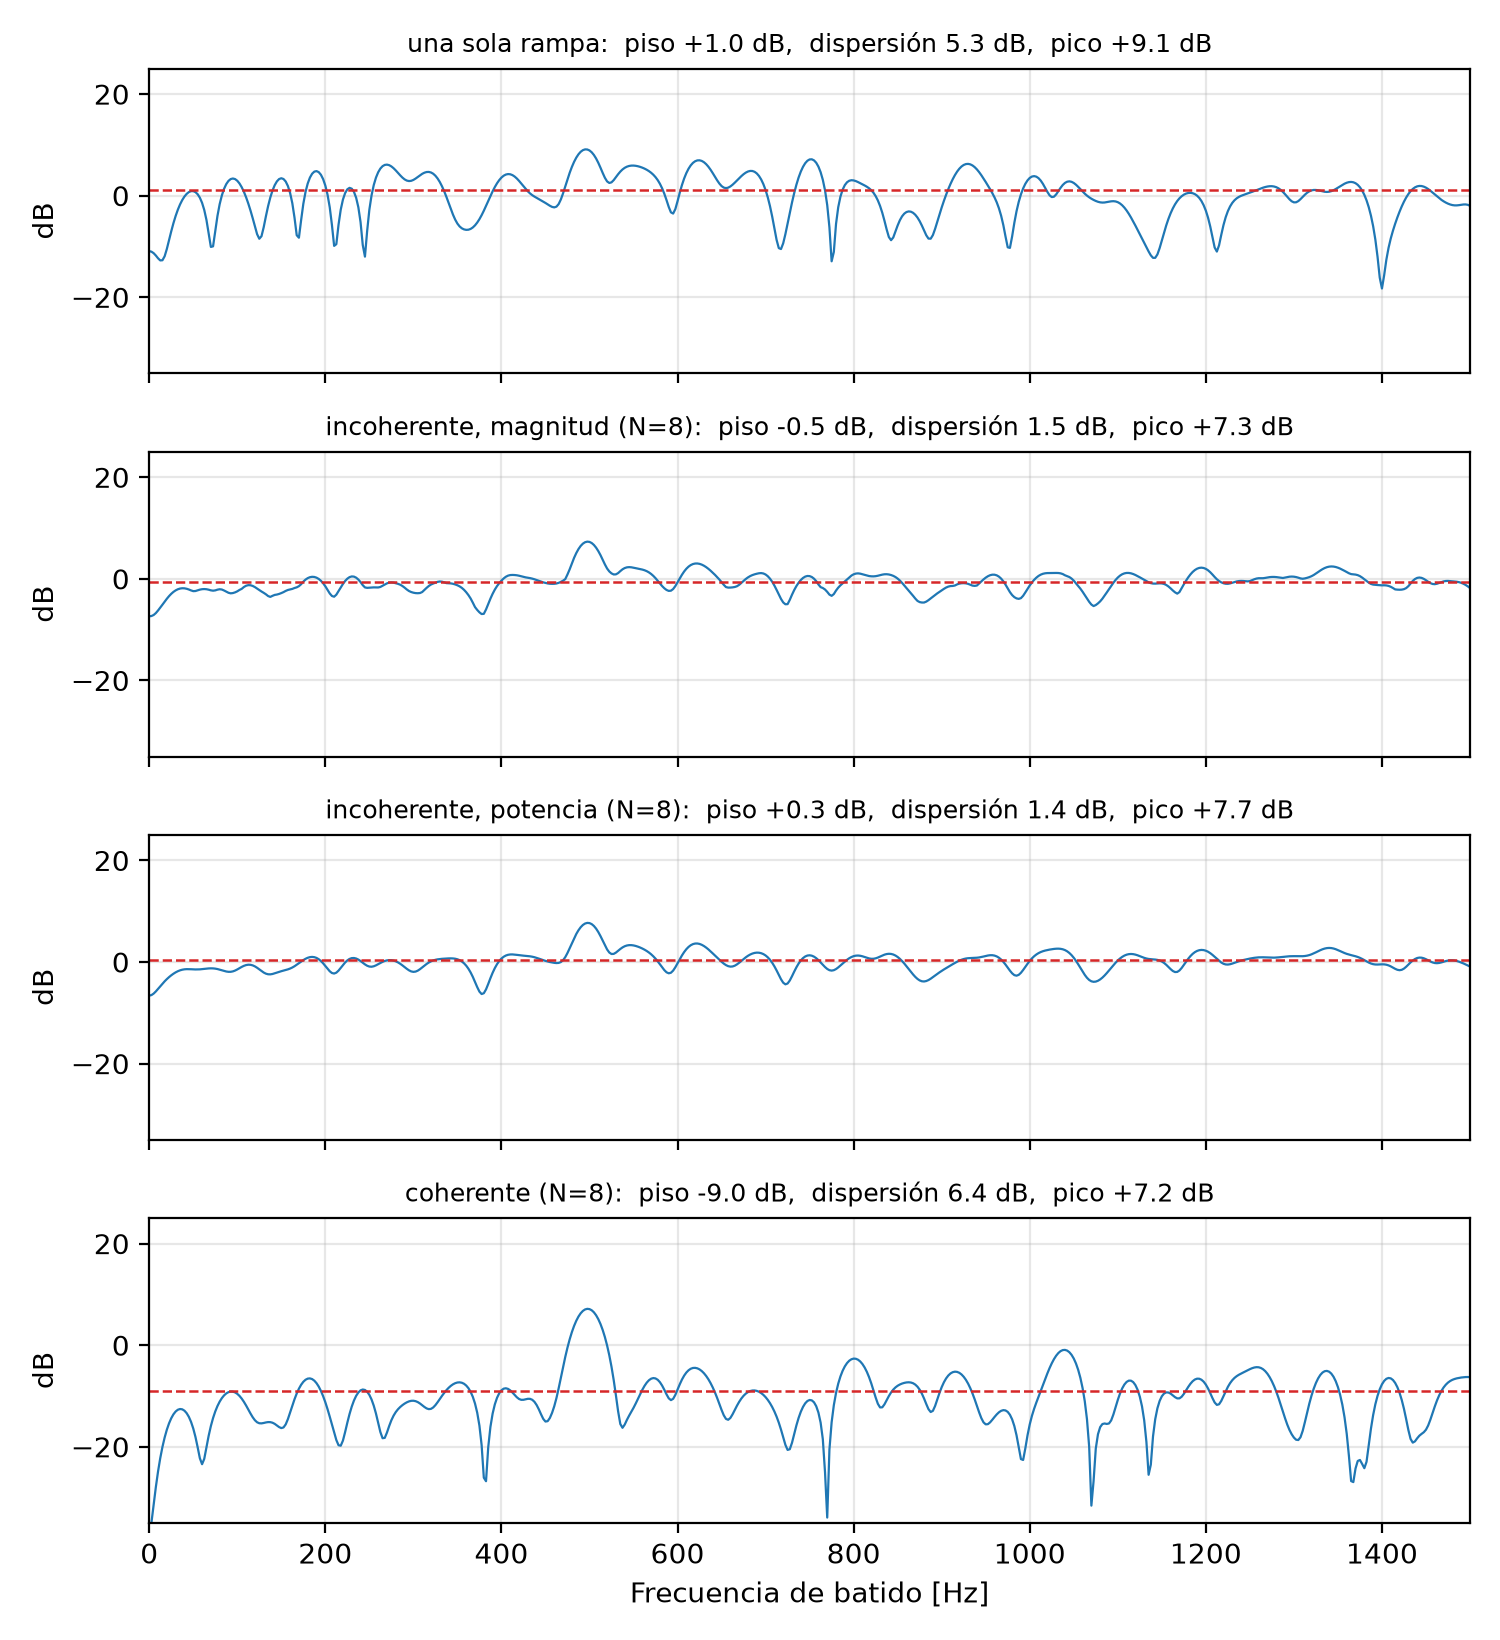
\includegraphics[width=0.92\linewidth]{figuras/procesamiento/promedio_espectros.png}
  \caption{Espectro de una fila de $N = 8$ rampas con un blanco débil en
  $498\,\text{Hz}$ (SNR de $-12\,\text{dB}$ por muestra en cada rampa),
  según el criterio de promedio. La línea roja es el piso medio. Una
  realización; los valores de los títulos varían entre corridas.}
  \label{fig:proc_espectros}
\end{figure}

La Figura~\ref{fig:proc_vs_N} separa las dos cosas que cambian con $N$: el
\emph{nivel} medio del piso y su \emph{dispersión}. El coherente sigue
exactamente la recta $-10\log_{10}N$ y no reduce la dispersión; el
incoherente reduce la dispersión como $1/\sqrt N$ y no mueve el nivel, salvo
un sesgo de hasta $-1{,}05\,\text{dB}$ cuando se promedia magnitud
(Sección~\ref{sec:proc_mag_pot}).

\begin{figure}[H]
  \centering
  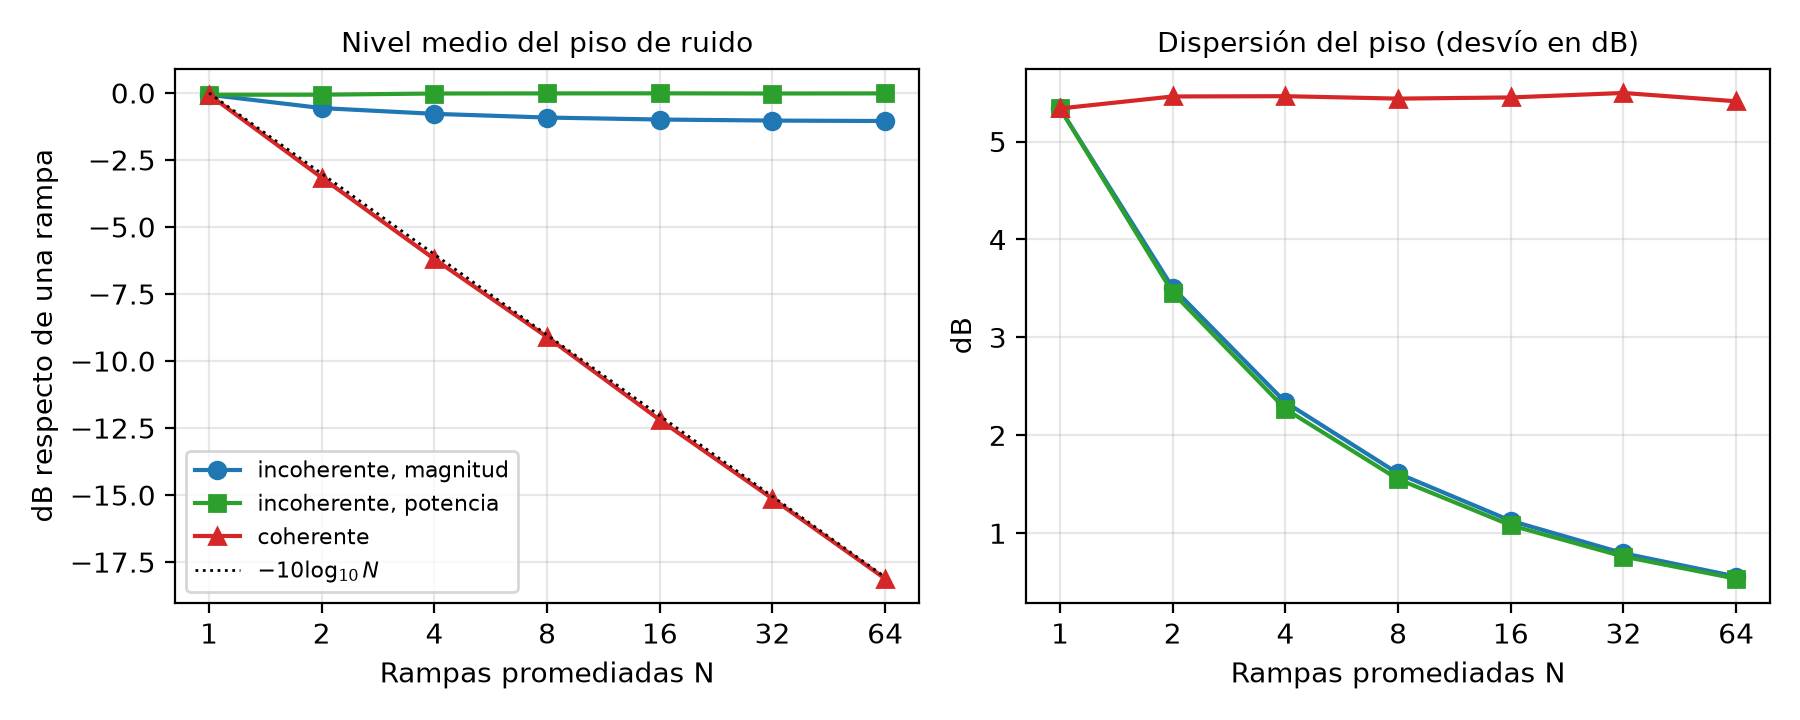
\includegraphics[width=\linewidth]{figuras/procesamiento/promedio_vs_N.png}
  \caption{Piso de ruido en función de la cantidad de rampas promediadas,
  sobre $300$ realizaciones de ruido puro. Izquierda: nivel medio, referido
  al de una rampa. Derecha: desvío del piso en dB a lo largo del espectro.}
  \label{fig:proc_vs_N}
\end{figure}

\subsection{Por qué el sistema usa el promedio incoherente}

La integración coherente rinde más, pero exige que \textbf{la fase del eco
se repita} de una rampa a otra, y en este banco eso no está garantizado:
\begin{itemize}
  \item \textbf{El sincronismo se reconstruye por software}
    (Sección~\ref{sec:proc_sincronismo}). Su error, de
    $\sim 10\,\mu\text{s}$, equivale a $\sim 2^\circ$ de fase a
    $500\,\text{Hz}$: pequeño, pero no medido sobre el banco real.
  \item \textbf{La repetibilidad del VCO entre barridos no está medida.}
    La fase del batido es $2\pi f(0)\tau + \dots$ (ecuación~\eqref{eq:proc_fase_batido}):
    una variación de $f(0)$ de una rampa a otra, por ruido de la
    triangular o deriva térmica del VCO, rota la fase del eco.
  \item \textbf{Subidas y bajadas tienen distinta fase.} Al invertir la
    bajada, el tono conserva la frecuencia pero no la fase. Un promedio
    coherente debería hacerse por separado para cada dirección.
  \item \textbf{Robustez.} Si la fase no se repite, el promedio coherente
    \emph{pierde} señal: en el límite de fases al azar, el eco también se
    cancela. El incoherente nunca pierde la señal.
\end{itemize}
Por eso se adopta el promedio incoherente: es el método estándar cuando no
se puede asegurar la coherencia de fase entre barridos \cite{Richards2014},
y el que ya se anticipaba en la Sección~\ref{sec:beat_freq} para combinar
subidas y bajadas. Verificar la estabilidad de fase sobre una captura cruda
y, si se confirma, pasar a un promedio coherente por dirección, queda como
trabajo futuro: se ganarían $\sim 9\,\text{dB}$ de piso con $N = 8$.

\subsection{Dónde se promedia}

El promedio~\eqref{eq:proc_incoherente} se usa en dos lugares, con dos $N$
distintos:
\begin{itemize}
  \item \textbf{Cada fila del radargrama}: $N$ rampas consecutivas. $N$ lo elige el
    usuario en el cuadro \texttt{rampas/col}; vale $8$ por defecto, una
    fila cada $0{,}4\,\text{s}$. El radargrama tiene la fila más nueva abajo y el
    tiempo hacia arriba (Figura~\ref{fig:proc_filas}). El espectro de la
    captura CSV es la última fila.
  \item \textbf{El perfil para el pico y la calibración}: las rampas de los
    últimos $2\,\text{s}$, unas $40$.
\end{itemize}
En memoria se guardan los perfiles de \emph{una} rampa, no las filas, así
que cambiar $N$ reagrupa todo lo que está en pantalla. Si la ventana pide
más de $900$ filas, que no entrarían en los píxeles del gráfico, $N$ se
agranda automáticamente y el panel lo informa como \emph{agrupado
efectivo}.

\begin{figure}[H]
  \centering
  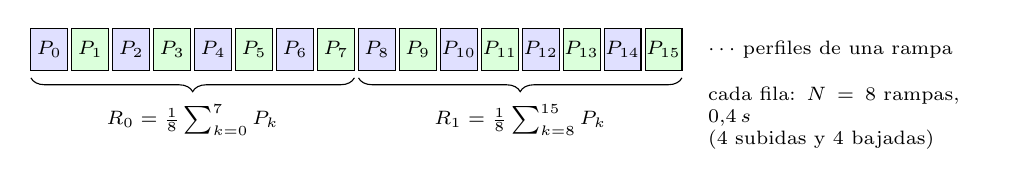
\begin{tikzpicture}[font=\scriptsize, x=0.52cm, y=0.6cm]
    \foreach \i in {0,...,15} {
      \ifodd\i \def\c{green!14}\else \def\c{blue!12}\fi
      \draw[fill=\c] (\i,0) rectangle (\i+0.9,0.9);
      \node at (\i+0.45,0.45) {$P_{\i}$};
    }
    \draw[decorate, decoration={brace, amplitude=5pt, mirror}]
      (0,-0.15) -- (7.9,-0.15) node[midway, below=6pt]
      {$R_0 = \frac{1}{8}\sum_{k=0}^{7} P_k$};
    \draw[decorate, decoration={brace, amplitude=5pt, mirror}]
      (8,-0.15) -- (15.9,-0.15) node[midway, below=6pt]
      {$R_1 = \frac{1}{8}\sum_{k=8}^{15} P_k$};
    \node[anchor=west] at (16.3,0.45) {$\cdots$ perfiles de una rampa};
    \node[anchor=west, text width=3.6cm] at (16.3,-1.0)
      {cada fila: $N = 8$ rampas, $0{,}4\,\text{s}$\\
       (4 subidas y 4 bajadas)};
  \end{tikzpicture}
  \caption{Formación de las filas del radargrama a partir de los perfiles de
  cada rampa. En azul las subidas, en verde las bajadas invertidas; cada fila
  mezcla las dos.}
  \label{fig:proc_filas}
\end{figure}

%------------------------------------------------------------
\section{Magnitud o potencia}
\label{sec:proc_mag_pot}

Dentro del promedio incoherente queda una elección: qué se promedia. Hay
tres opciones habituales:
\begin{align}
  \text{lineal (magnitud):}\quad   & \textstyle \frac{1}{N}\sum_k \lvert X_k\rvert,
  \label{eq:proc_lineal}\\
  \text{cuadrática (potencia):}\quad & \textstyle \frac{1}{N}\sum_k \lvert X_k\rvert^2,
  \label{eq:proc_cuadratica}\\
  \text{logarítmica:}\quad          & \textstyle \frac{1}{N}\sum_k 20\log_{10}\lvert X_k\rvert.
  \label{eq:proc_log}
\end{align}
El sistema usa la lineal y convierte a decibeles después del promedio, con
$20\log_{10}$. Los criterios para elegir dependen de para qué se usa el
resultado.

\subsection{Para detectar y ubicar el pico, da lo mismo}

En la teoría de detección con integración incoherente, el detector lineal
(suma de $\lvert X_k\rvert$) y el cuadrático (suma de $\lvert X_k\rvert^2$)
difieren normalmente en \textbf{menos de $0{,}2\,\text{dB}$} de
rendimiento. El cuadrático es algo mejor con relación señal a ruido baja y
el lineal con relación alta \cite{Richards2014, Skolnik2001}. Además, la
posición del máximo es la misma con cualquiera de los tres criterios, porque
las tres operaciones son monótonas. Para la función principal del radar,
estimar distancias, la elección no pesa.

\subsection{Para medir niveles, la potencia es la correcta}

Cuando lo que interesa es un \emph{nivel} (el piso de ruido, la energía de
la puerta de detección, la comparación con la simulación o entre capturas),
los tres criterios no dan lo mismo.

\paragraph{La potencia es el estimador sin sesgo.}
Promediar $\lvert X_k\rvert^2$ es el periodograma promediado de Bartlett y
Welch, el estimador estándar de la densidad espectral de potencia
\cite{Welch1967, Proakis2006}: su valor esperado es la potencia verdadera, y
su varianza baja aproximadamente $N$ veces.

\paragraph{La magnitud subestima el ruido.}
Por~\eqref{eq:proc_rayleigh}, para un bin de ruido
\begin{equation}
  \frac{\bigl(\operatorname{E}\lvert\eta\rvert\bigr)^2}
       {\operatorname{E}\lvert\eta\rvert^2} = \frac{\pi}{4}
  \quad\Longrightarrow\quad
  10\log_{10}\frac{\pi}{4} = -1{,}05\,\text{dB}.
  \label{eq:proc_sesgo_mag}
\end{equation}
Un tono fuerte casi no fluctúa y no sufre ese sesgo. El resultado es que,
promediando magnitudes, \textbf{la relación pico/piso sale hasta
$1{,}05\,\text{dB}$ más optimista} que la real. El sesgo crece con $N$: es
nulo con una rampa, porque $\lvert X\rvert^2$ de una sola rampa ya es
potencia, y vale $-0{,}92\,\text{dB}$ con $N = 8$
(Figura~\ref{fig:proc_vs_N}).

\paragraph{El promedio en decibeles subestima más.}
Promediar en escala logarítmica subestima la potencia del ruido en
$10\log_{10}(e)\,\gamma = 2{,}51\,\text{dB}$, con $\gamma$ la constante de
Euler. Es el error clásico de los analizadores de espectro con promedio de
video en escala logarítmica \cite{KeysightAN150}. El sistema no promedia en
decibeles.

\paragraph{La potencia es aditiva.}
Para señal y ruido no correlacionados,
$\operatorname{E}\lvert s + \eta\rvert^2 = \lvert s\rvert^2 + \sigma^2$.
Esa propiedad es la que da sentido estadístico a restar un fondo, o un piso
de ruido, de un espectro promediado. Las magnitudes no se suman así.

Los tres sesgos se verificaron con la simulación de Monte Carlo: dio
$-1{,}05\,\text{dB}$ y $-2{,}50\,\text{dB}$, contra $-1{,}05$ y
$-2{,}51\,\text{dB}$ teóricos.

\subsection{Qué implica para el sistema}

\begin{itemize}
  \item \textbf{Las distancias no se ven afectadas.} El pico, la traza del
    radargrama y la calibración no cambian con el criterio.
  \item \textbf{Los niveles de ruido en pantalla están $\sim 1\,\text{dB}$
    por debajo de su valor verdadero}, y la relación pico/piso $\sim
    1\,\text{dB}$ por encima.
  \item \textbf{La puerta de detección mezcla los criterios}: calcula la
    energía como suma de cuadrados (Sección~\ref{sec:proc_fondo}), pero de
    magnitudes ya promediadas en lineal.
  \item \textbf{La comparación con la simulación} se hace sobre curvas
    normalizadas a su propio máximo (columna \texttt{db\_norm} de la CSV
    de captura), y un sesgo constante del piso no cambia la posición ni la
    forma de los picos.
\end{itemize}
Pasar a un promedio de potencia, mostrado con $10\log_{10}$, es un cambio
menor en el código que dejaría todos los niveles sin sesgo. Mientras no se
haga, los niveles absolutos de ruido que se informen deben corregirse por el
sesgo~\eqref{eq:proc_sesgo_mag}.

%------------------------------------------------------------
\section{Sustracción del fondo y detección}
\label{sec:proc_fondo}

\subsection{Fondo congelado}

Sin ningún blanco, la pantalla no queda vacía: el acoplamiento directo entre
antenas, la pared del laboratorio y el resto de la sala producen ecos fijos.
Con la sala vacía, el botón \emph{medir fondo} promedia $3\,\text{s}$ de
perfiles y guarda
\begin{equation}
  F[\ell] = \frac{1}{K}\sum_{k} P_k[\ell].
\end{equation}
Desde ese momento, a cada fila se le resta el fondo, con piso en cero:
\begin{equation}
  D_r[\ell] = \max\bigl(R_r[\ell] - F[\ell],\; 0\bigr).
  \label{eq:proc_resta_fondo}
\end{equation}
La referencia de $0\,\text{dB}$ pasa a ser el pico del fondo en la zona útil,
fija, en vez del máximo de la pantalla. Esto evita que, sin blanco, el propio
fondo suba a $0\,\text{dB}$ y aparezca un pico donde no hay nada.

La resta~\eqref{eq:proc_resta_fondo} es entre \emph{magnitudes}, porque es
lo único que se guarda. Una resta de complejos cancelaría un eco fijo de
forma exacta; una resta de magnitudes lo atenúa, pero no puede separar un
blanco del fondo cuando caen en el mismo bin con fases que se restan. Es una
limitación aceptada de la integración incoherente.

\subsection{Puerta de detección}

Se declara que hay un blanco sólo si la energía actual, en la zona por
encima de la distancia mínima $d_\text{ign}$, supera a la del fondo en un
margen:
\begin{equation}
  E = \sum_{\ell \geq \ell_0} R[\ell]^2,
  \qquad
  10\log_{10}\frac{E}{E_F} \geq \text{margen}\quad (6\,\text{dB}).
\end{equation}
Si no se cumple, el programa informa \emph{sin blanco} en vez de una
distancia. Antes de agregar la puerta, con la sala vacía el sistema
informaba igual la distancia del eco más fuerte del fondo.

\subsection{Fondo automático (MTI)}

Como alternativa, el fondo puede estimarse de forma continua con un promedio
exponencial:
\begin{equation}
  F \leftarrow F + a\,\bigl(\bar P - F\bigr),
  \qquad a = 1 - e^{-\Delta t/\tau_\text{MTI}},
  \qquad \tau_\text{MTI} = 30\,\text{s},
\end{equation}
donde $\bar P$ es el promedio de las rampas del último refresco y $\Delta t$
su duración. Es un filtro pasaaltos en el tiempo lento: lo que no se mueve
termina adentro de $F$ y desaparece, y lo que aparece o se mueve resalta
durante $\sim\tau_\text{MTI}$. Con el fondo automático la puerta compara la
energía del \emph{residuo} $\max(R - F, 0)$ contra la del fondo, porque la
energía cruda coincide con la del fondo por construcción.

\subsection{Distancia del pico}

El pico se busca en el perfil de los últimos $2\,\text{s}$, con el fondo ya
restado, a partir de $d_\text{ign}$ ($0{,}3\,\text{m}$): por debajo está el
acoplamiento directo, que es lo más fuerte de todo el espectro. Sobre el
bin del máximo, $\ell^*$, y sus dos vecinos se ajusta una parábola en
decibeles \cite{Jacobsen2007}:
\begin{equation}
  \delta = \frac{1}{2}\,\frac{a - c}{a - 2b + c},
  \qquad
  \hat d = d_{\ell^*} + \delta\,\Delta d,
  \label{eq:proc_parabola}
\end{equation}
con $a$, $b$, $c$ los niveles en dB de los bins $\ell^*-1$, $\ell^*$ y
$\ell^*+1$, $\Delta d$ el paso de la grilla y
$\lvert\delta\rvert \leq 1/2$. Se usa la escala en dB porque, cerca del
máximo, el lóbulo principal de la ventana de Hann es casi una parábola en
dB. Sobre tonos sintéticos, el error de posición baja de $0{,}22$ bins a
prácticamente cero. Esto no cambia la resolución, que sigue siendo
$c/(2B)$: mejora la precisión con que se ubica el centro de un pico ya
resuelto, que es lo que hace repetible un punto de calibración.

Finalmente, la distancia aparente se lleva a distancia real con la
calibración afín del Capítulo~\ref{ch:cables},
$d_\text{real} = a\,\hat d + b$, donde $b$ es el offset de los cables y
$a$ debe dar $\approx 1$.

%------------------------------------------------------------
\section{Ejemplo: placa a 90 cm}
\label{sec:proc_ejemplo}

La Figura~\ref{fig:proc_radargrama} es una captura del programa con una
placa metálica a $90\,\text{cm}$ y el fondo congelado. Arriba, el
radargrama: $50$ filas de $N = 8$ rampas ($0{,}4\,\text{s}$ cada una) que
cubren $20\,\text{s}$, con la frecuencia de batido en el eje horizontal. La
traza roja es el pico de cada fila. Abajo, el espectro de la última fila en
dB sobre el fondo; el pico está en $498\,\text{Hz}$, que
por~\eqref{eq:proc_eje} son $3{,}59\,\text{m}$ aparentes: $0{,}9\,\text{m}$
de aire más el offset de cables y bocinas. La energía supera al fondo en
$8{,}2\,\text{dB}$, por encima del margen de $6\,\text{dB}$, así que la
puerta declara blanco. A la derecha, el panel con el estado completo de la
cadena (período ajustado, $F_\theta$, $B$, $\alpha_0$, resolución) y la
triangular plegada sobre el período ajustado.

\begin{figure}[H]
  \centering
  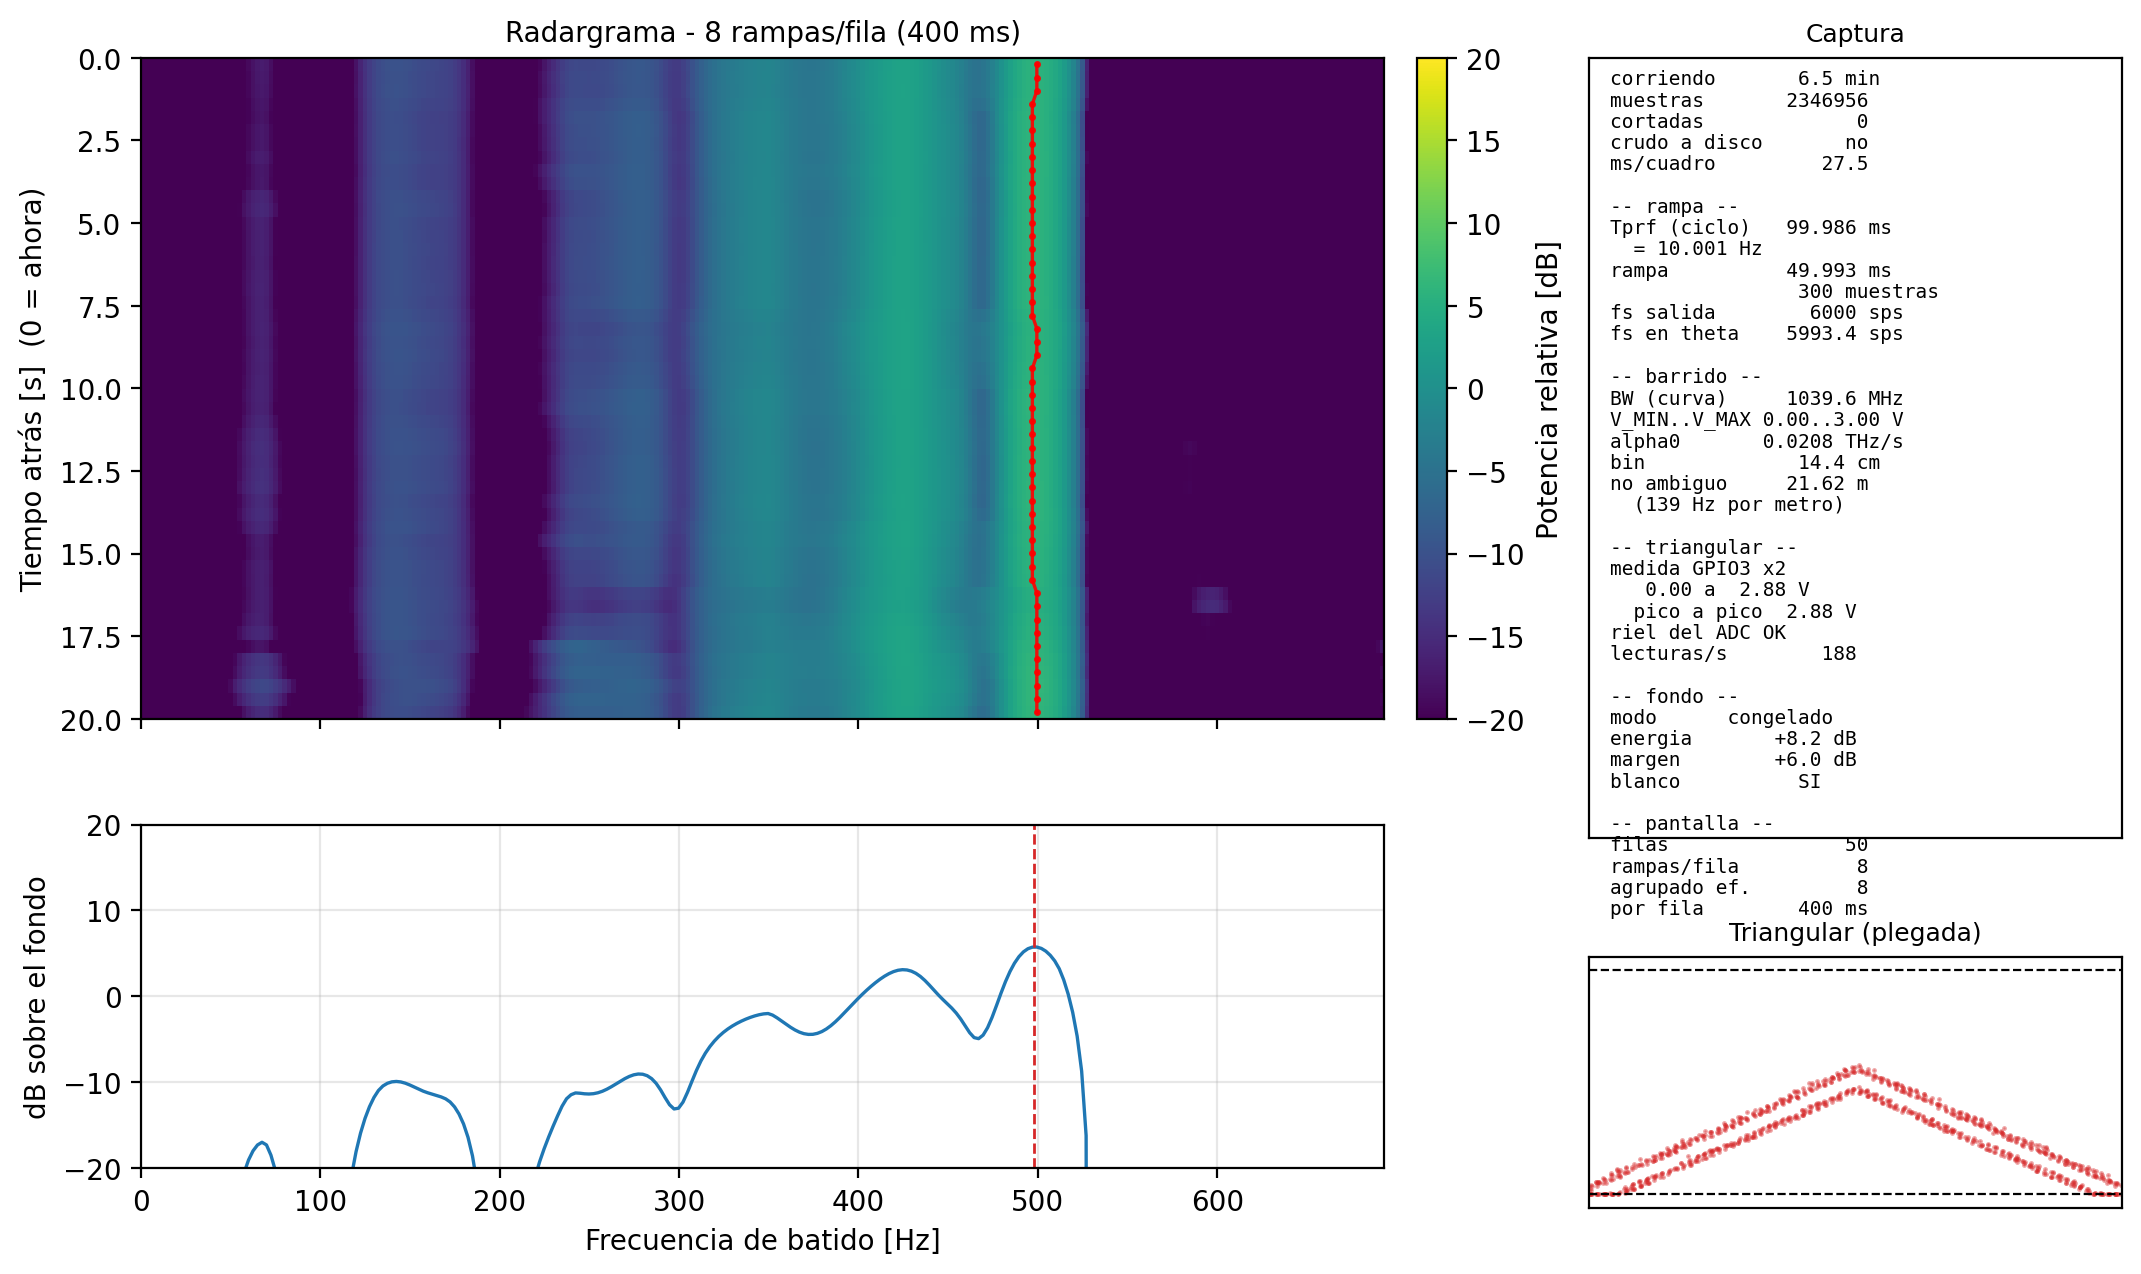
\includegraphics[width=\linewidth]{figuras/procesamiento/radargrama_placa_90cm.png}
  \caption{Captura de \texttt{vivo\_rapido.py} con una placa metálica a
  $90\,\text{cm}$, fondo congelado, $N = 8$ rampas por fila (28/09/2026).}
  \label{fig:proc_radargrama}
\end{figure}

%------------------------------------------------------------
\section{Resumen de la cadena}
\label{sec:proc_resumen}

\begin{table}[H]
  \centering
  \caption{Etapas del procesamiento, con su ecuación y su implementación.}
  \label{tab:proc_resumen}
  \small
  \begin{tabular}{>{\raggedright\arraybackslash}p{2.9cm}
                  >{\raggedright\arraybackslash}p{6.0cm}
                  >{\raggedright\arraybackslash}p{5.2cm}}
    \toprule
    \textbf{Etapa} & \textbf{Operación} & \textbf{Dónde} \\
    \midrule
    Diezmado & semibanda $\times 3$, $48\,\text{k}\to 6\,\text{k}$,
      ec.~\eqref{eq:proc_diezmado} & \texttt{adquisicion.ino} (firmware) \\
    Sincronismo & máx.\ de $\lvert S(T)\rvert$ y fase,
      ecs.~\eqref{eq:proc_armonico}--\eqref{eq:proc_fase}
      & \texttt{ajustar\_\allowbreak triangular\_\allowbreak rapido()} \\
    Corte de rampas & ec.~\eqref{eq:proc_limites}, bajadas invertidas
      & \texttt{Vivo.procesar()} \\
    Resta de la media & $\tilde x = x - \bar x$ & \texttt{Vivo.procesar()} \\
    Corrección del VCO & remuestreo a $\theta$ uniforme,
      ecs.~\eqref{eq:proc_theta}--\eqref{eq:proc_fs_theta}
      & \texttt{Remuestreador} \\
    Ventana y FFT & Hann, $N_\text{FFT} = 2400$, ec.~\eqref{eq:proc_fft}
      & \texttt{espectros()} \\
    Perfil & $P_k = \lvert X_k\rvert$, ec.~\eqref{eq:proc_perfil}
      & \texttt{espectros()} \\
    Promedio & incoherente, en magnitud,
      ec.~\eqref{eq:proc_incoherente} & \texttt{Vivo.matriz()} \\
    Fondo & ec.~\eqref{eq:proc_resta_fondo} o MTI
      & \texttt{Vivo.matriz()} \\
    Pico & parábola en dB, ec.~\eqref{eq:proc_parabola}
      & \texttt{pico\_parabolico()} \\
    Distancia & ec.~\eqref{eq:proc_eje} y calibración afín
      & \texttt{Calibracion} \\
    \bottomrule
  \end{tabular}
\end{table}

\section{Conclusiones del capítulo}
\label{sec:proc_conclusiones}

\begin{itemize}
  \item \textbf{El sincronismo existe y es de software.} Se reconstruye
    ajustando un período y una fase a $\sim 50$ períodos de la triangular
    leída por GPIO3. El error en el límite de rampa queda en
    $\sim 10\,\mu\text{s}$, menos de una décima de muestra.
  \item \textbf{Cada FFT es de una sola rampa de $50\,\text{ms}$}, subida o
    bajada invertida. Las dos mitades del triángulo duplican las rampas
    útiles, $20$ por segundo.
  \item \textbf{El remuestreo en $\theta$ convierte el batido de un VCO no
    lineal en un tono puro} (ec.~\eqref{eq:proc_tono_theta}), y es el que
    permite que el pico tenga el ancho que le corresponde por la
    resolución, $c/(2B) = 14{,}4\,\text{cm}$.
  \item \textbf{Las rampas se integran de forma incoherente.} El piso de
    ruido no baja, pero su dispersión cae como $1/\sqrt N$ (de $5{,}3$ a
    $1{,}6\,\text{dB}$ con $N = 8$). Se eligió así porque la coherencia de
    fase entre barridos no está garantizada en este banco. El promedio
    coherente rendiría $\sim 9\,\text{dB}$ más con $N = 8$, y queda como
    trabajo futuro una vez verificada la estabilidad de fase.
  \item \textbf{Se promedia magnitud, no potencia.} Para ubicar picos es
    indistinto (diferencia menor a $0{,}2\,\text{dB}$ en detección y
    ninguna en posición); para medir niveles, el piso queda
    $\sim 1\,\text{dB}$ subestimado.
\end{itemize}
